\section{Einleitung\label{Kap.:Einleitung}}

Die analoge Welt wird immer digitaler, mit dem Einzug der Mikroelektronik wurden analoge Messvorrichtungen durch meist präzisere, digitale Sensoren ersetzt. Dieses Konzept zieht sich durch alle Bereiche des Lebens. Mit dem Aufkommen und der starken Verbreitung von leistungsfähigen Endgeräten, wie Computer, Smartphone oder Tablet und der massiv voranschreitenden Vernetzung verschiedenster Komponenten, hält auch die Digitalisierung Einzug in alltägliche Bereiche und Tätigkeiten wie beispielsweise dem Kochen.

Innerhalb dieser Dokumentation wird die Entwicklung einer smarten Küchenwaage beschrieben. Die smarte Küchenwaage zeichnet mit einem durchgängigem Integrierungskonzept in den normalen Alltag des Nutzers aus. Hierfür muss die Waage einfach bedienbar, die Grundfunktionalitäten einer normalen Küchenwaage und erweiterte, smarte Funktionen aufweisen. Zu den Grundfunktionen einer Waage wird im Folgendem das Anzeigen des aktuellen Gewichtes verstanden. Um die Waage smarten Funktionen zugänglich zu machen, wird einen Schnittstelle benötigt, über diese Schnittstelle kann der Nutzer mit der Waage interagieren und erweiterte Funktionen aufrufen. Die Waage besteht im Grundaufbau aus verschiedenen Hardwarekomponenten, welche in Kapitel \ref{Kap.:Hardware} vorgestellt werden, an dieser Stelle wird auch der prinzipielle Aufbau der Waage beschrieben. Neben der Hardware, muss die Waage ebenfalls mit der passenden Software ausgestattet sein, welche die Hardwarekomponenten korrekt ansteuert und so den reibungslosen Ablauf garantiert, dies wird in Kapitel \ref{Kap.:Software} dargestellt. 

Innerhalb des Kapitels \ref{Kap.:Zusammenfassung} wird der aktuelle Entwicklungsstand der Waage aufgezeigt und weitere smarte Funktionalitäten in Form eines Ausblicks dargestellt. 

\section{Hardwareaufbau\label{Kap.:Hardware}}
Im Folgenden werden verschiedene Lösungskonzepte miteinander verglichen um eine smarte Küchenwaage aufzubauen.%TODO: evtl. etwas ausschmücken

\subsection{Lösungskonzept}

Um eine smarte Küchenwaage mit erweiterten Funktionalitäten aufzubauen bestehen mehrere Möglichkeiten.
\begin{itemize}
	\item[1.]  Eine bestehende smarte Küchenwaage reverse-engineeren und deren Übertragungssignal abfangen und manipulieren um hierauf eine eigene Anwendung aufzubauen 
	\item[2.] eine normale Küchenwaage nutzen, diese mit einem Microcontroller ausstatten und den gemessenen Wert übertragen 
	\item[3.] Aufbauen einer eigenständigen Lösung mithilfe verschiedener Sensoren und Aktoren
\end{itemize}

Die Hauptaufgabe innerhalb des ersten Szenarios liegt darin zu verstehen, wie die genutzte bestehende smarte Küchenwaage arbeitet, den Messwert aus der Datenübertragung zu extrahieren und anschließend mit diesem eine Anwendung aufzusetzen, welche weitere Features implementieren kann.

Das zweite Szenario ist hingegen schon wesentlich komplexer, hier muss das Signal über bestehende Leiterbahnen abgefangen werden. Eine besondere Herausforderung besteht darin diese zuerst freizulegen und den normalen Messvorgang nicht zu beeinflussen. Anschließend muss eine Schnittstelle aufgebaut werden, um den Nutzer weitere Funktionen zugänglich zu machen. 

Mit dem eigenen Aufbau einer smarten Küchenwaage bestehen die meisten Freiheiten, so können die Komponenten beliebig gewählt und ausgetauscht werden, auch muss keine bestehende Lösung adaptiert werden. Jedoch besteht darin auch die besondere Herausforderung, die schiere Größe des Projekts. Hier muss nicht nur der Client aufgebaut werden, auch muss die komplette Waage selbst erstellt und getestet werden. Hierfür müssen bestehende Lösungen evaluiert werden. Diese macht diesen Ansatz jedoch auch so interessant, da hier mit der Hardware direkt gearbeitet werden und so ein tieferes Verständnis über diese und den genutzten Technologien erworben werden kann. 

Es ist zu beachten, dass innerhalb aller Szenarien eine Schnittstelle für erweiterte Funktionalitäten benötigt wird, diese kann lokal durch zum Beispiel einem großen Bildschirm oder extern über eine Schnittstelle zu einem mobilem Endgerät bereitgestellt werden. Da davon ausgegangen werden kann, dass jeder Nutzer einer smarten Küchenwaage auch ein Handy oder Tablet besitzt, wird sich für die Lösung einer Softwareschnittstelle entschieden, da diese kostengünstiger implementiert werden kann. Mehr hierzu wird unter Kapitel \ref{Kap.:BLE} beschrieben.

\begin{figure}[hbtp]
	\centering
	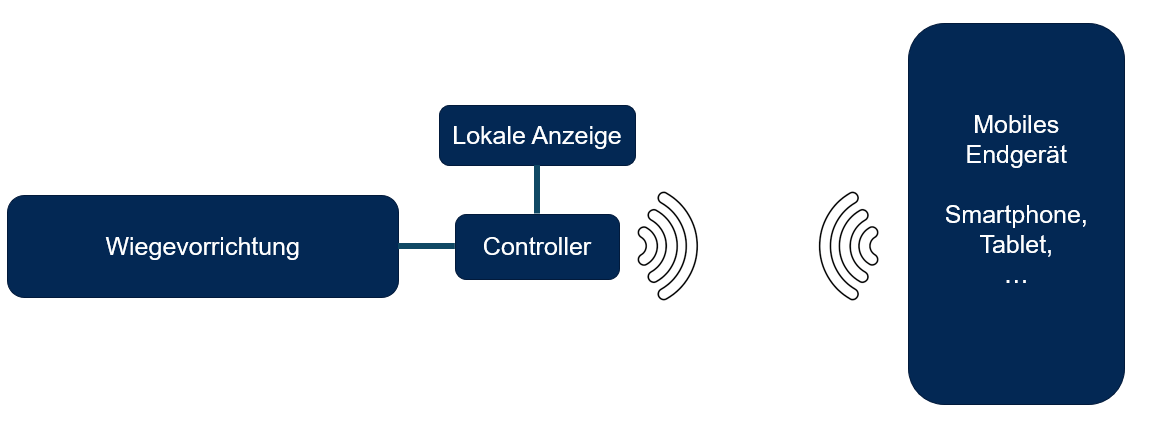
\includegraphics[width=1\textwidth]{Bilder/HW-Aufbau.png}
	\caption{Aufbau der smarten Küchenwaage}
	\label{fig.:HW-Aufbau}
\end{figure}
Da mit der Erstellung einer eigenen Küchenwaage die meisten Freiheiten und das größte Lern-Potential ist, wurde sich für diesen Weg entschieden. Der allgemeinen Systemaufbau ist in Abbildung \ref{fig.:HW-Aufbau} dargestellt. Um ein Objekt zu wiegen benötigt es eine zentrale Wiegevorrichtung, welche über einen Mikrocontroller angebunden ist, die lokale Anzeige des Gewichts übernimmt ein separates Bauteil. Über den Mikrocontroller selbst oder einem eigenständigen Bauteil soll die Kommunikation  mit einem mobilen Endgerät aufgebaut werden. 


\subsection{Controller}

Der Controller der smarten Waage sollte möglichst kostengünstig sein und einen geringen Stromverbrauch aufweisen um gegebenenfalls auch mit einer Batterie betrieben werden zu können. Aus diesem Hintergrund wird ebenfalls zur Kommunikation mit dem mobilen Endgerät \ac{BLE} verwendet. Bestehende Möglichkeiten für den Controller sind somit die Mikroprozessoren von Arduino oder RaspberryPi.
Da die Aufgabe der Prozessoren lediglich in der Messwerterfassung, Anzeige und Übertragung liegt, scheint der RaspberryPi überdimensioniert. In der Familie der Arduino-Mikroprozessoren sind die folgenden Boards mit Bluetooth ausgestattet: 
\begin{itemize}
	\item Nano IOT
	\item Nano BLE
	\item Nano BLE Sense
	\item BT
	\item Genuino 101
	\item MKR VIDOR 4000
\end{itemize}

Ebenso besteht die Möglichkeit ein eigenes Bluetooth-Modul wie das  HM10 BLE 4.0 anzuschließen, da nur ein sehr kompakter Bauraum vorhanden ist (siehe Kapitel \ref{Kap.:Wiegevorrichtung}), wird sich zur Auswahl auf die zuvor beschriebenen Boards beschränkt, im speziellen auf die kleinen Nano Boards. Da das Messen der Umgebung nicht gebraucht wird, entfällt der BLE Sense, eine finale Größe des Codes ist noch nicht vorhersehbar, weshalb sich für den Nano BLE entschieden wird, da dieser einen größeren Speicher besitzt. 


\subsection{Wiegevorrichtung\label{Kap.:Wiegevorrichtung}} 

Zur Aufnahme des Gewichts wird eine Wiegevorrichtung benötigt, diese setzt sich aus Sensor zur Messung des Gewichts, Standbein und Plattform für den zu messenden Gegenstand zusammen. 

Innerhalb der Wägetechnik werden oft Wäghezellen verwendet, diese bestehen aus einem Federkörper mit Dehnungsstreifen. Über diese kann ein analoges Signal erzeugt werden, welches auf die über der Wägezelle abgeleiteten Masse schließen lässt. Mittels eines Digital Analog Konverters, im speziellem dem HX711, kann ein digitales Signal erzeugt werden und an den Arduino zur Weiterverarbeitung gesendet werden.

Die Wägezelle selbst ähnelt einem Quader, welcher über eine Seite mit einem Fuß und auf der anderen mit der Plattform befestigt wird. Um das Messen komfortabel zu gestalten, wurden zwei baugleiche Teile entworfen und mithilfe von einem 3D-Drucker erzeugt. Die Entwürfe der Teile sind in Abbildung \ref{fig.:3D-Druck} dargestellt.

\begin{figure}[hbtp]
	\centering
	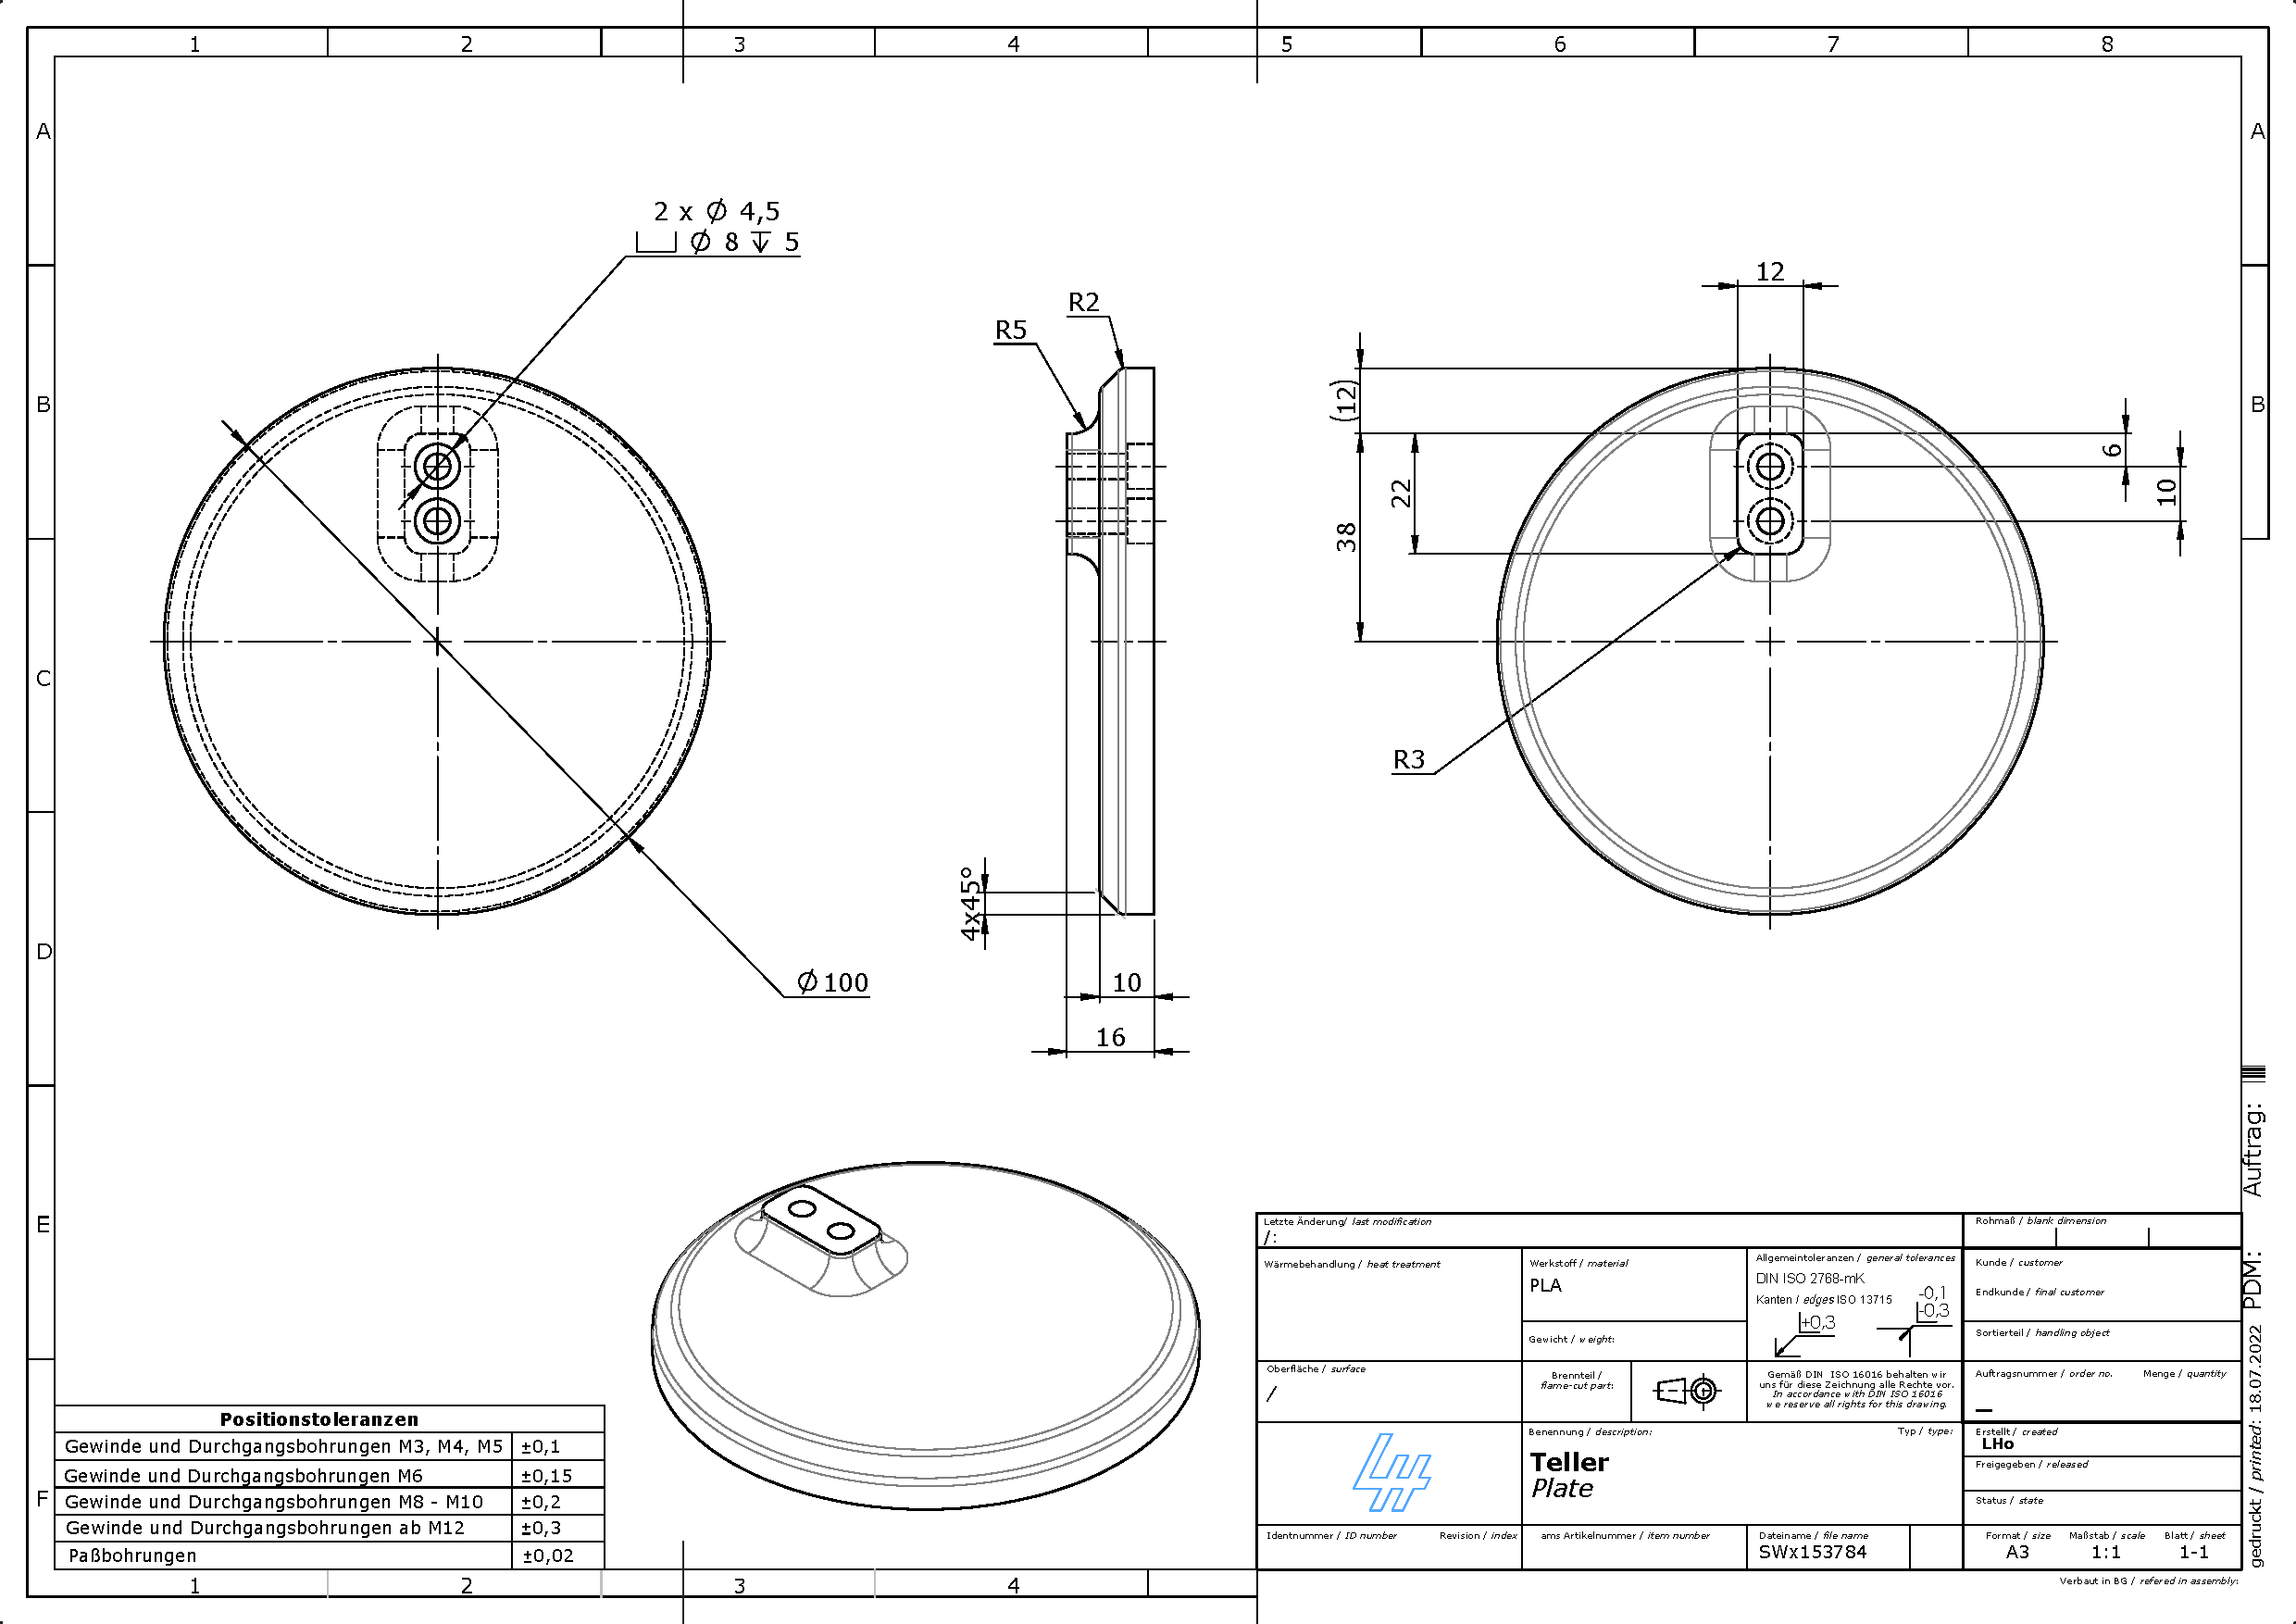
\includegraphics[width=1\textwidth]{Bilder/Teller-1.pdf}
	\caption{Entwurf des Fußes und der Wägeplattform der Waage}
	\label{fig.:3D-Druck}
\end{figure} 

Die Erhöhung ist nötig, um der Wägezelle zum messen genügend Spiel einzuräumen. Das Bauteil wird zweimal gedruckt und horizontal, sowie vertikal um 180 Grad entgegengesetzt an der Zelle angebracht, zu sehen in Abildung \ref{fig.:System}.

\begin{figure}[hbtp]
	\centering
	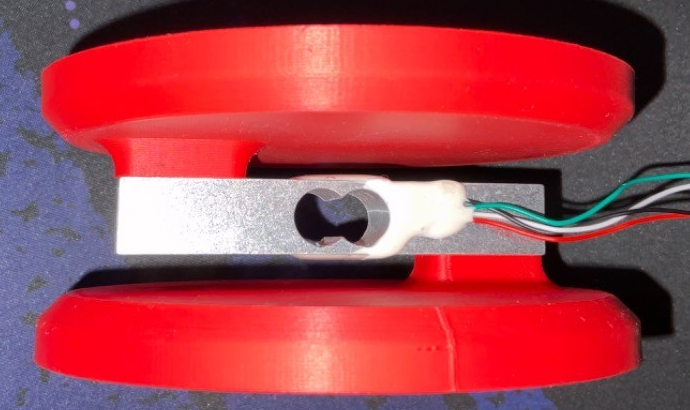
\includegraphics[width=1\textwidth]{Bilder/System.png}
	\caption{Die 3D gedruckten Teile sind mit M4-Schrauben an der Wägezelle befestigt, hierzu wurde eine Aussparung an der Unterseite der Teile für die Schrauben gelassen.}
	\label{fig.:System}
\end{figure} 

\subsection{lokale Anzeige}

Um die Küchenwaage auch ohne mobilem Endgerät nutzen zu können, wird eine Anzeige des aktuellen Gewichts benötigt, die Wägezelle hat ein Maximalgewicht von 10 kg, da beim Backen oder Kochen die Menge der Zutaten teilweise sehr genau bestimmt werden muss, sollte die Anzeige mindestens 4 stellen besitzen um bis auf 9999 g grammgenau wägen zu können. Um die Hardwarekosten sowie den Stromverbrauch der Waage möglichst gering zu halten, wird eine 7 Segmentanzeige mit 4 Stellen verbaut.  

\subsection{Verbinden der Komponenten}

Die soeben vorgestellten Komponenten müssen nun mit dem Controller verbunden werden. Für die prototypische Umsetzung wird mithilfe eines Steckbretts gearbeitet, in einem finalen Produkt kann der 3D-Druck jedoch so angepasst werden, dass die Komponenten zwischen Fuß und Messvorrichtung untergebracht und verkleidet werden. Die physische Verbindung der Komponenten ist in Abbildung \ref{fig.:Frizzing} zu sehen.

\begin{figure}[hbtp]
	\centering
	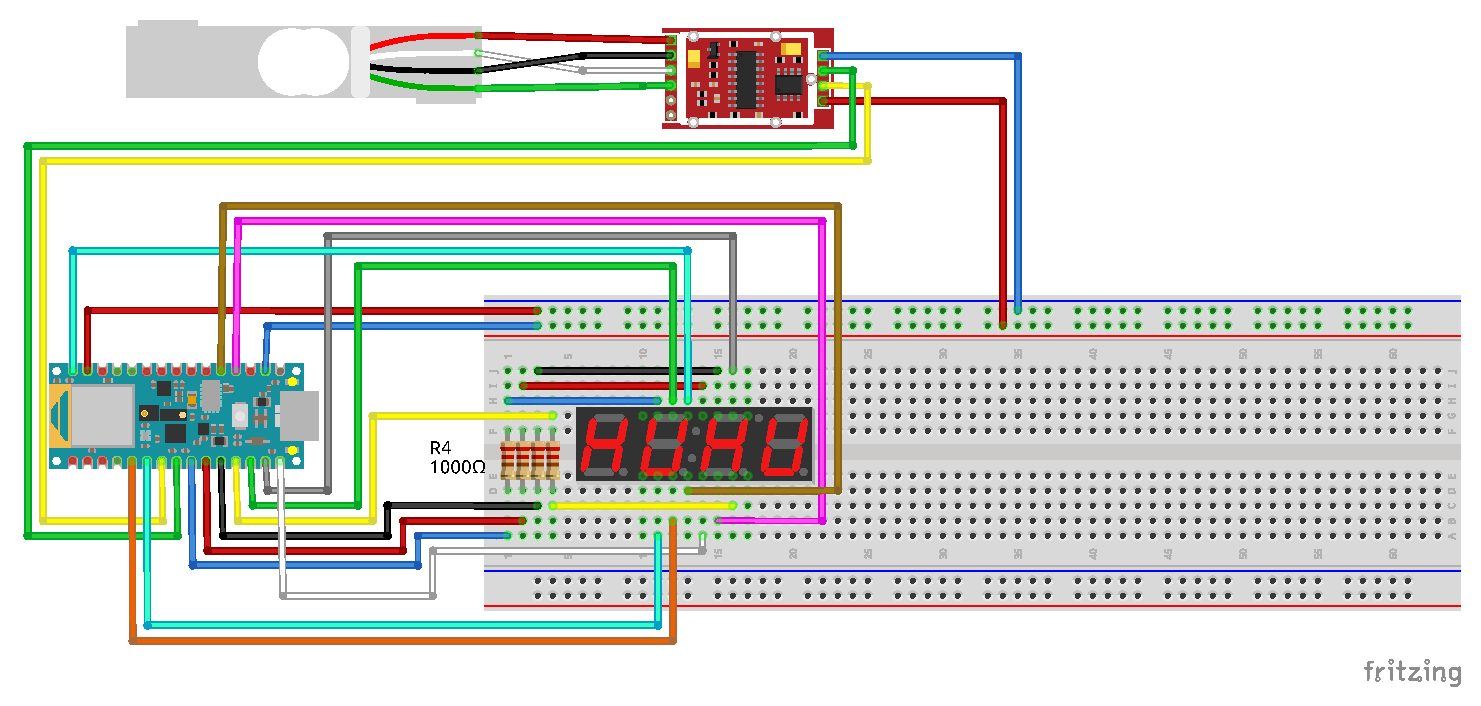
\includegraphics[width=1\textwidth]{Bilder/Platinenlayout.pdf}
	\caption{Die Komponenten sind mit dem Arduino verbunden, sollte im Folgenden Kapitel \ref{Kap.:Software} auf Pins eingegangen werden, entspricht dies der hier abgebildeten Verkabelung.}
	\label{fig.:Frizzing}
\end{figure} 

\section{Software\label{Kap.:Software}}

Mit dem Zusammenstellen der Komponenten wird nun die passende Software benötigt, diese teilt sich auf in Software für den Microcontroller und für das mobile Endgerät.

\subsection{Arduino}
Essentiell für den Erfolg des Projektes ist die Datenerfassung, Datenvorverarbeitung und Datenübertragung vom Microcontroller, da verschiedene Hardwarekomponenten verwendet werden, wird der Programmcode seperat beschrieben und anschließend zu einem Sketch zusammengeführt. 

\subsubsection{Wägezelle}

Die Wägezelle ist wie bereits beschrien mit einem Digital Analog Converter verbunden, dieser wird neben der Spannungsversorung über 3,3 V und Ground mit zwei digitalen Pins des Arduions verbunden, wobei einer der Pins zur Regelung des Taktes und die andere zur Signalübertragung genutzt wird. Z

um Auslesen des Sensors wird die Bibliothek HX711.h verwendet. 
Nach dem initialen tarieren der Waage mit einem bekannten Gewicht, was idealerweise 50\% des zulässigen Gesamtgewichts der Waage schwer ist, kann das aktuelle Gewicht mit nur einem Funktionsaufruf bestimmt werden. Um nicht unnötig oft zu messen, die Anzeige nicht unnötig schnell zu aktualisieren und so den Nutzer gegebenenfalls zu verwirren, wird der Messvorgang nur einmal pro Sekunde ausgeführt und auf 1 Gramm gerundet.
\subsubsection{BLE\label{Kap.:BLE}}

Da sich bewusst für ein Controller mit eingebauter \ac{BLE}-Funktionalität entschieden wurde, wird diese Funktechnologie zur Datenübertragung an die mobilen Endgeräte verwendet. \ac{BLE} bietet hierbei die Vorteile eines einfachen Publish-Subscribe Mechanismus um von Base zum Client sich zu Verbinden und eine Übertragung so von der Waage nur dann zur Base aufzubauen, wenn diese einen neuen Wert gemessen hat. Außerdem liegt ein weiterer Vorteil von \ac{BLE} in der stromeffizienten Übertragung.

Prinzipiell baut \ac{BLE} auf Services auf, welche wiederum Charakteristiken mit Übertragungsformaten haben. Für die smarte Küchenwaage ist prinzipiell nur das Abfragen und Subscriben auf einen Wert nötig, den des gemessenen Gewichts. Beim Verbindungsaufbau mit dem Board wird eine eigene Schleife aufgerufen, welche solange aktiv ist, wie die Bluetooth Verbindung besteht, so kann sich bei einmaligem Einschalten der Waage jederzeit ein Smartphone verbinden und trennen von der Waage. 

\subsubsection{Segmentdisplay}
Das Segmentdisplay wird durch Multiplexing angesteuert,  So wird für die 4 Nummern, bestehend aus 7 Segmenten nur 12 Pins benötigt, welche sich auf 4 Nummern-Pins und 8 Segment Pins zusammensetzen. 
Das Aufrufen und Updaten des Displays muss für eine kontinuierliche Anzeige der Werte stets innerhalb der normalen Schleife und innerhalb des \ac{BLE}-Loops geschehen, da andernfalls die Anzeige dunkel bleibt und kein Wert angezeigt wird. 

\subsection{App}

Zur Erweiterung der normalen Wägefunktionen muss eine Schnittstelle geschaffen werden, welche es erlaubt anhand des gemessen Wertes weitere Interaktionen auszuführen, da zur Datenübertragung BLE genutzt wird, muss das Endgerät auf dem die Schnitttstelle laufen soll \ac{BLE} ebenfalls unterstützen. Die meisten modernen Smartphones und Tablets tun dies. 
Aus diesem Grund wird eine App entwickelt, welche auf den Plattformen iOS und Android lauffähig seien soll, hierzu werden im Folgenden verschiedene Entwicklungsmöglichkeiten betrachtet zur Programmierung von Apps betrachtet 
\subsubsection{Framework}
Zur Entwicklung von Apps existieren vier Möglichkeiten 
\begin{itemize}
	\item Native Entwicklung
	\item native Cross Plattform Entwicklung
	\item Hybride Entwicklung 
	\item Progressive Web Apps
\end{itemize}

Bei der nativen Entwicklung werden für iOS und Android jeweils eine eigene Codebase verwendet, es muss also für beide Betriebssysteme eine eigenen App entwickelt werden.

Native Cross Platform Apps setzen auf eine zwischengeschaltete Programmiersprache, um mithilfe eines Frameworks wie Xamarin native Anwendungen zu erzeugen. Somit kann ein Großteil der Codebase werden um native Apps zu generieren, Nachteile ergeben sich jedoch innerhalb des Userinterfaces, welches vollständig durch ein eigenes Rendering des Frameworks überschrieben wird.

Hybride Apps sind in Webanwendungen, welche mittels eines Frameworks in einem nativen Container für die Zielplattform überführt werden, dadurch können hybride Apps auf native APIs der Zielplattform zugreifen

Progressive Web Apps ähnlen stark hybriden Apps, jedoch werden diese in einer Browserumgebung ausgeführt und klönnen dennoch offline genutzt werden.

Anhand der dargestellten Merkmale wird sich für das Einsetzen von einem hybriden Entwicklungsanstaz entschieden, da dieser gut auf die Hardware des Gerätes, also das Bluetooth-Modul,zugreifen kann und direkt iOS, Android und eine Web-Browser Version unterstützt werden können. 

Auf Grund erster Erfahrung in Angular wird das Framework Ionic verwendet. Unter Zuhilfenahme von Capacitor und Android Studio kann so eine Android App entwickelt werden. 
 
\subsubsection{BLE}

Capacitor wird mithilfe eines Community-Plugins um eine \ac{BLE}-Schnittstelle erweitert. Diese Schnittstelle ermöglicht das erkunden nach neuen BLE-Geräten mit spezifischen Eigenschaften, spo kann in der Anwendung nutzerfreunlich nur die eigene \ac{BLE}-fähige Waage angezeigt werden. Wird sich mit der Waage nun verbunden, so wird an die App mithilfe der festgelegten \ac{BLE}-Service Charakteristik der aktuelle Messwert an die Mobile-App übertragen. dieser kann anschließen zur weiteren Berechnung verwendete und ausgegeben werden.

\subsubsection{Mobile App}

Die Frontendentwicjlung gestaltet sich ähnlich der, einer Angular Anwendung. verschiedene Module sind unterschiedlichen Routen zugeordnet, welche über ein Hauptfenster bedinet werden können. Ionic bringt verschiedene erste Layouts mit, in der Anwendung wird sich für ein Tabs Moidul entschieden, welches am unteren Seitenrand mehrere Tabs zur Hauptnavigation hat. Innerhalb des ersten Tabs ist eine normale Waagenfunktionalität nachgenbaut, hier wird lediglich das Gewicht angezeigt. Über die anderen Tabs können anschließenden Iterationen weitere Funktionalitäten liefern. 

\section{Zusammenfassung und Ausblick \label{Kap.:Zusammenfassung}}

Mit der ersten Implementierung einer smarten Küchenwaage konnten einige Ziele erreicht werden, jedoch bietet die Küchenwaage noch keine zusätzlichen smarten Features, der aktuelle Entwicklungsstand wird im Folgendem diskutiert und mögliche Erweiterungen dargestellt.


\subsection{Reflexion}% (Takt-, BLE-, … Probleme)

In der ersten Implementierungsiteration konnte erfolgreich ein erster Prototyp einer smarten Küchenwaage aufgebaut werden. Hierfür wurde sich an bestehen Lösung der Wägetechnik, energiesparsamen Kommunikation und zeitgemäßer App Entwicklung bedient. 

Dennoch ist der erste Prototyp nicht perfekt, durch die hohen Anforderungen von Bluetooth, dem zyklischem Messen der Waage und dem aktualisieren des Segmentdisplays scheint der Controller teilweise überlastet, was sich durch ein sichtbares Flimmern am Segmentdisplay ableiten lässt. 

Die verwendeten Elektronikkomponenten liegen zum aktuellen Zeitpunkt noch frei und sind nicht in einem Gehäuse verbaut. 

Mit dem Fehlen einer Nullungs-Funktion am Controller selbst fehlt eine typische Funktion einer handelsüblichen Küchenwaage, so kann das Tarrieren nur bei Systemstart vollzogen werden. 

Da während des zeitlich limitierten Entwicklungsprozesses die Funktionalität der Waage im Vordergrund stand, benötigt diese noch eine feste Stromquelle, das einplanen und einbauen von Batterien oder wenigstens eines Akkus sollte in künftigen ENticklungsprozsses berücksichtigt werden.

\subsection{Ausblick} %(bessere Teller für die Waage, smartes Kochbuch, Foodtacker, Social Funktionen, …)

Wie bereits zuvor beschrieben, hat der Prototyp ein hohes Potential bezüglich weiterer Entwicklungen. Nachfolgend werden einige Gedanken dargestellt.

\textbf{Physische Erweiterungen}

Die smarte Küchenwaage sollte in späteren Entwicklungsstufen ohne externe Stromquelle und in dem üblichen Umfeld arbeiten können. Hierfür ist es notwendig die Waage mit einer Stromquelle auszustatten und das Gehäuse der Waage so anzupassen, dass dieses zumindest gegen Spritzwasser geschützt ist. Eine Lösung für das Display, der Ladefunktion und eine Nullungsfuktion muss noch erarbeitet werden. 

\textbf{Softwareerweiterungen}

Wie schon oft in dieser Ausarbeitung angesprochen, liegt das größte Potential der Waage innerhalb der Software. 

So ist es denkbar, ein smartes Kochbuch zu implementieren, welches den Nutzer durch den gesamten Zubereitungsprozess leitet. Für das Hinzufügen von Zutaten kann die Softwar die benötigte Zutat und die noch benötigte Menge berechnen und diese auf dem Smartphone ausgeben. Sollte der Nutzer den Zielwert stark überschreiten, kann die Anwendung vorschlagen die Menge der anderen Zutaten anzupassen oder Teile der Zutat vom Nutzer entnehmen lassen. 

Ebenfalls kann die Waage zum Tracken der Ernährung helfen, so kann eine Datenbank an die App angebunden werden, über welche sich Nährwerte berechnet werden können und ein digitales Tage-Kochbuch geführt werden kann.
 
 Das zuvor beschrieben Kochbuch kann auch von den Nutzern bearbeitet und erweitert werden. So kann der Nutzer beispielsweise neue Gerichte für sich lokal anlegen, diese exportieren und mit Freunden teilen, mögliche social Funktionen sind auch denkbar, so kann dies womöglich direkt in der App selbst geschehen.
